% Vision Models Are More Robust And Fair When Pretrained On Uncurated Images Without Supervision: https://arxiv.org/pdf/2202.08360v2.pdf

% Metodologia: Explicação detalhada do método de pesquisa utilizado (quantitativa, qualitativa, estudo de caso, revisão sistemática etc.).

% Contextualização: Apresentação do contexto ou cenário relacionado ao tema (histórico, cultural, social, econômico, entre outros).

% Treinamento, Classificação

% Análise de Dados/Resultados: Apresentação, descrição e interpretação dos dados coletados ou das análises realizadas.

% Discussão: Comparação dos resultados com a literatura existente, reflexões e implicações teóricas ou práticas.

% Limitações da Pesquisa: Identificação de possíveis limitações no estudo, como escopo, recursos ou tempo.

% O Google Colab é um serviço do Jupyter Notebook hospedado que oferece acesso gratuito a recursos de computação, incluindo GPUs e TPUs. Ele é adequado principalmente para aprendizado de máquina, ciência de dados e educação. 

\chapter{Desenvolvimento}
\label{cap:03}

\section{MMF}

O MMF, é um framework modular para pesquisa de visão e linguagem multimodal de código aberto criado pelo Facebook AI Research (FAIR). É considerado o estado da arte (state-of-the-art) desse seguimento, onde foi utilizado como referência para desenvolver projetos como o Visualbert.

Já o Detectron2 é uma plataforma também de código aberto para detecção de objetos, segmentação e outras tarefas de reconhecimento visual. Também é considerado o estado da arte em detecção e segmentação, onde oferece suporte a vários projetos de pesquisa de visão computacional.

PyTorch é uma biblioteca de aprendizado de máquina em código aberto usada para implementações de aprendizado profundo, como visão computacional (usando TorchVision) e processamento de linguagem natural

\begin{figure*}[!htbp]
	\centering
	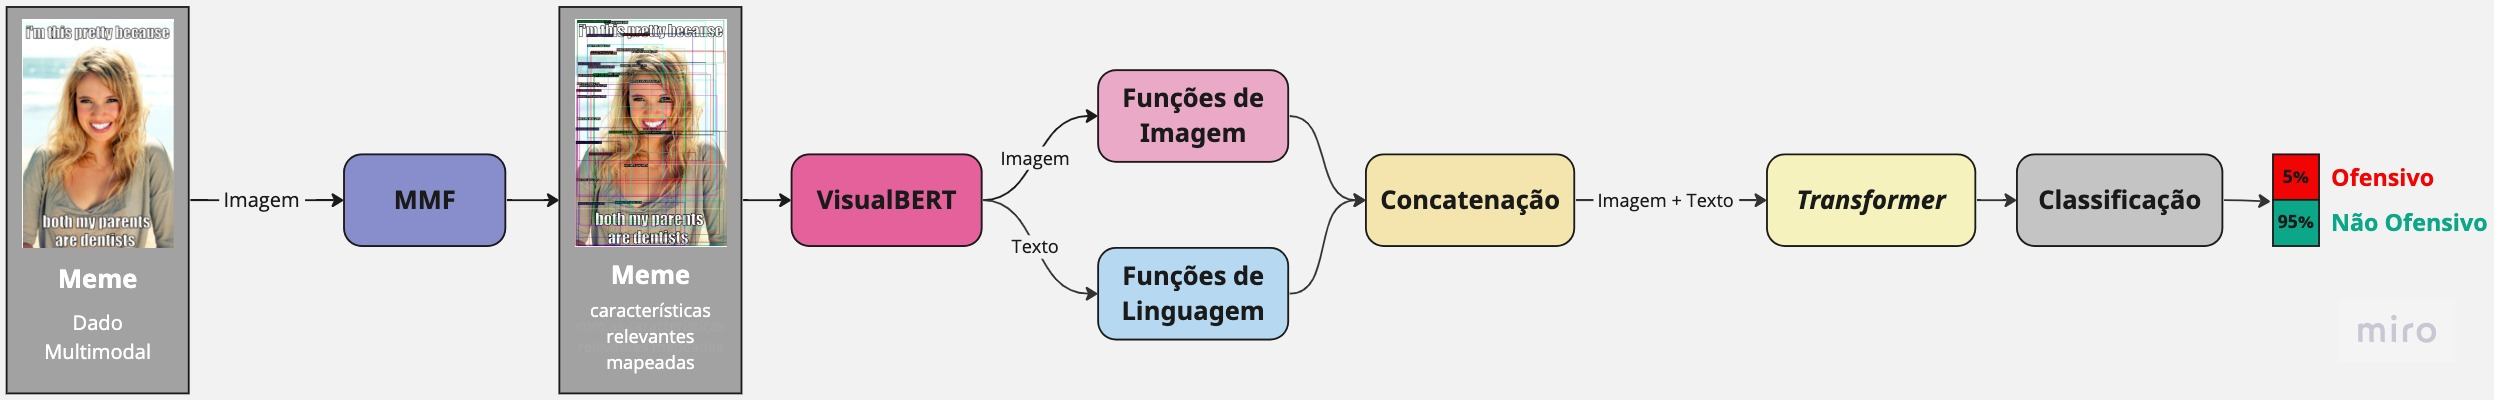
\includegraphics[scale=0.18]{imagens/diagrama.jpeg}
    \caption {Arquitetura da Proposta de Desenvolvimento.}
\end{figure*}


% \section{Proposta}

% Para iniciar o projeto, será utilizado o banco de dados de memes odiosos criado pela Meta, composto por 10 mil memes em inglês que contêm conteúdo ofensivo relacionado a gênero, raça, religião, orientação sexual, classe social e outros tópicos. Dada à sensibilidade desses dados, eles só estão disponíveis para pesquisas que estejam em conformidade com os termos de uso referentes a sua utilização, compartilhamento e armazenamento. O conjunto de dados é composto pelas seguintes porcentagens: 40\% de memes de ódio multimodal, 10\% de memes de ódio unimodal, 20\% de memes com confusão de texto benigna, 20\% de memes com confusão de imagem benigna e 10\% de memes não odiosos aleatórios. Os ``confundidores benignos'' consistem em imagens ou textos alternativos para cada meme odioso, que alteram sua classificação para não odioso. Esses confundidores foram adicionados para garantir que o conjunto de dados seja apropriado para testar a verdadeira capacidade multimodal de um modelo, levando em conta que, no mundo real, o modelo se depararia com exemplos diversos e inéditos.

% Dando sequência no desenvolvimento do trabalho, será utilizado o modelo MMF, uma estrutura pré-definida com funcionalidades para pesquisa multimodal de visão e linguagem fornecida pelo \textit{Facebook AI Research}\footnote{MMF: \textit{a framework for vision-and-language multimodal research from Facebook AI Research} (FAIR). 2020. Disponível em: \url{https://github.com/facebookresearch/mmf}. Acesso em: 24 de mai. de 2023.}. Esse modelo será aplicado para detectar objetos e extrair características relevantes das imagens presentes no banco de dados, seu funcionamento consiste em receber uma imagem de entrada e produzir uma coleção de caixas delimitadoras, cada uma contendo um objeto identificado, juntamente com sua categoria, como por exemplo, animal ou humano. Essa abordagem visa aprimorar o desempenho do \textit{VisualBERT}, um modelo já pré-treinado com um vasto conjunto de dados de legenda e imagem.

% O conjunto de dados de memes odiosos não tem o propósito de treinar o modelo do \textit{VisualBERT} a partir do zero, mas sim de ajustá-lo e testá-lo, a fim de reduzir o viés e possibilitar uma identificação e classificação mais eficiente de memes considerados como odiosos ou ofensivos. Para atingir esse objetivo, será utilizado o método de aprendizagem supervisionada, combinado com o aprendizado profundo e por conjuntos, utilizando a métrica primária de área sob a curva característica de operação do receptor (AUROC) e a acurácia para avaliar a eficiência e a precisão do modelo, o objetivo é alcançar métricas com um valor igual ou superior a 0,7.


% % A AUROC é uma medida que avalia a capacidade do modelo em distinguir corretamente as classes positiva e negativa, enquanto a acurácia mede a proporção de predições corretas em relação ao total de predições. Essas métricas serão fundamentais para garantir a qualidade e confiabilidade dos resultados obtidos pelo modelo.

% A etapa de treinamento e aprendizado onde serão os maiores desafios do projeto, pois requer ajustes finos usando a rede neural aprendida como base para obter melhores resultados no processo de reconhecimento de padrões. A cada certa atualização do modelo é realizada uma nova avaliação no conjunto de validação, utilizando uma taxa de aprendizado definida para controlar as etapas de atualização de treinamento durante o ajuste fino. Uma pesquisa de hiperparâmetros é conduzida para encontrar a configuração ideal, na qual o modelo é avaliado com diferentes conjuntos de hiperparâmetros, considerando suas pontuações de AUROC. Por fim, a técnica de votação majoritária é aplicada para realizar a classificação binária final dos memes multimodais, distinguindo entre os ofensivos e não ofensivos. 

% % O ajuste fino é uma técnica comum em aprendizado profundo que envolve a adaptação de um modelo pré-treinado a uma tarefa downstream específica, treinando-o em dados específicos da tarefa. O modelo VisualBERT ajustado é então usado para fazer previsões sobre novos memes. Além disso, o projeto usa aprendizado conjunto, que é uma técnica que combina as previsões de vários modelos para melhorar o desempenho. A abordagem de conjunto usa vários modelos de aprendizado profundo que são ajustados em diferentes subconjuntos dos dados de treinamento para melhorar o desempenho geral do sistema.

% % Por fim, a abordagem aplica aprendizado conjunto para combinar as previsões de vários modelos para melhorar o desempenho. A abordagem alcançou um AUROC de 0,811 e uma precisão de 0,765 no conjunto de teste de desafio

% % Fazer pré-treinamento em grandes conjuntos de dados reduz a variância, mas aumenta o viés. Além disso, aumentar o tamanho do conjunto de dados nem sempre melhora o desempenho. Por exemplo, [80] observaram que o tamanho do conjunto de dados não é o fator mais importante no pré-treinamento visual-linguístico. Eles afirmam que mesmo um conjunto de dados menor pode facilmente superar o pré-treinamento em um conjunto de dados maior quando o domínio visual e textual correto corresponde a dados de boa qualidade.

% % Realizamos uma extensa pesquisa de hiperparâmetros e usamos a melhor configuração para os parâmetros, incluindo taxa de aprendizado, etapas de aquecimento, tipo de aquecimento, fator de aquecimento e iterações de aquecimento. Avaliamos os modelos com diferentes hiperparâmetros durante a busca da grade e os 27 melhores modelos, de acordo com suas pontuações AUROC, são conjuntos. Finalmente, a técnica de votação por maioria é aplicada para finalizar a classificação.

% \section{Cronograma}

% Como forma de organizar e alcançar os objetivos deste trabalho no próximo semestre, será adotada a metodologia SCRUM, um \textit{framework} ágil utilizado no gerenciamento de projetos, especialmente no desenvolvimento de \textit{software} \cite{MicheleSligerSCRUM}. É conhecido por promover a flexibilidade e adaptabilidade, permitindo uma resposta ágil a mudanças e prioridades. E com base nessa metodologia, o trabalho será organizado adaptando os ciclos característicos do SCRUM para melhor atender às necessidades do projeto.

% \begin{figure*}[!htbp]
% 	\centering
% 	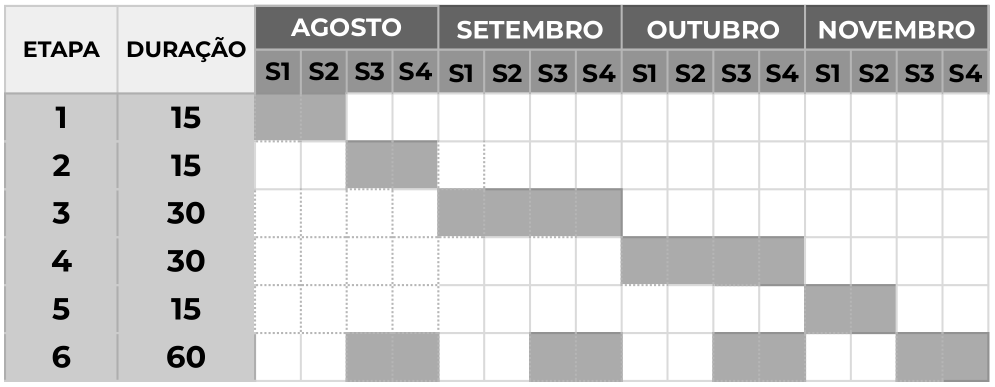
\includegraphics[scale=0.9]{imagens/cronograma}
%     \caption {Cronograma proposto: \textbf{Etapa 1.} Extração de características relevantes das imagens do banco de dados; \textbf{Etapa 2.} Utilização do modelo do \textit{VisualBERT}; \textbf{Etapa 3.} Treinamento; \textbf{Etapa 4.} Classificação dos memes; \textbf{Etapa 5.} Testes, análises e levantamento dos resultados; \textbf{Etapa 6.} Documentação.}
% \end{figure*}

% O trabalho será dividido em seis etapas, em que cada uma delas terá uma lista de tarefas que incluirão funcionalidades, requisitos e melhorias a serem implementadas. Para organizar o desenvolvimento do projeto, serão adotados ciclos chamados \textit{sprints}, com duração de 2 semanas. No início de cada \textit{sprint}, um conjunto de tarefas será selecionado para desenvolvimento dentro do prazo estabelecido, utilizando o método \textit{Kanban}, onde as tarefas serão divididas em colunas representando as etapas de ``a fazer'', ``em desenvolvimento'' e ``concluídas''. E ao final de cada \textit{sprint}, planejo fazer uma revisão do trabalho realizado para identificar pontos de melhoria e ajustes para os próximos \textit{sprints}. Esses pontos poderão ser compartilhados e discutidos em conjunto com o orientador do trabalho.

% Detalhando melhor as etapas do cronograma, a primeira \textit{sprint} irá começar com a utilização do \textit{framework} MMF para extrair características relevantes das imagens do banco de dados de memes odiosos, juntamente com o preparo do ambiente de desenvolvimento. Após a utilização e familiaridade com a ferramenta, a próxima \textit{sprint} será dedicada à utilização do modelo \textit{VisualBERT} com as imagens já tratadas pelo MMF. Em seguida, serão necessárias duas sprints para realizar o treinamento, em seguida mais duas \textit{sprints} para a classificação dos memes com base nesse treinamento. Após a conclusão dessas etapas, será realizada uma \textit{sprint} de testes e análises dos resultados obtidos, e caso necessário, haverá a possibilidade de retornar às etapas de treinamento e classificação para realizar melhorias adicionais. Além disso, será feito um levantamento de todos os resultados interessantes, que serão apresentados e detalhados. Por fim, a cada uma \textit{sprint}, a documentação será atualizada com o passo a passo detalhado de como as etapas foram realizadas, garantindo um registro claro e organizado do progresso e das decisões tomadas ao longo do projeto.